%\documentclass [twoside,12pt]{article}
\documentclass[11pt,twocolumn]{article}
\usepackage{amsmath}
\usepackage{mathtools}
\usepackage{braket}
\usepackage{latexsym}
\usepackage{graphicx}
\usepackage{fullpage}
\usepackage[switch]{lineno}
\usepackage{hyperref}
\usepackage{subcaption}
\usepackage{lipsum}
\graphicspath{{images/}}

\begin{document}
%\linenumbers

\twocolumn[
\begin{@twocolumnfalse}
\title{Muon lifetime}
\author{Christina Nelson \\
University of Hawaii Manoa \\
canelson@hawaii.edu}
\date{March 24, 2017}
\maketitle

\begin{abstract}
A muon ``telescope'' is built with plastic scintillators and photomultiplier tubes to observe cosmic ray flux at sea-level. Measured flux per solid angle is approximately $(0.023 \pm 0.001)$ s$^{-1}$cm$^{-2}$sr$^{-1}$; due to low statistics, this deviates from the accepted value of $0.07$ s$^{-1}$cm$^{-2}$sr$^{-1}$. Statistics are increased by extending the duration of data acquisition. Accurate measurements are obtained for muon lifetime $\tau_{\mu} = (2.19 \pm 0.12)$ $\mu$s, and a clear observation of the zenith angular dependence $\propto cos(\theta)^2$ is also found.


\indent\indent
\end{abstract}
\indent
\indent
\end{@twocolumnfalse}
]
\indent \indent
This month marks the $80^{th}$ anniversary of the discovery of muons from cosmic ray showers, made by Caltech physicists Carl D. Anderson and Seth Neddermeyer. Anderson and Neddermeyer measured the energy loss from cosmics using a platinum plate in a cloud chamber and observed two distinct groups of particles: one with high absorption, and another that penetrated through the platinum and lost little energy. \cite{anderson} The first group of particles were known to be electrons, while the latter suggested a different particle with a mass almost $200$ times heavier than the electron. At first the penetrating particles were interpreted as mesons, a hypothetical particle at the time predicted by theorist Hideki Yukawa. About a decade later Italian physicists determined that the detected particle first seen by Anderson and Neddermeyer was actually a decay product from a $\pi$ meson, and the leptonic particle became known as the muon.\cite{hyper}\cite{encyc}

\indent \indent
Muons are interesting particles that are important in many areas of physics research and may help in deepening our understanding of nature and the Universe. Their discovery pointed to the three generations that form the Standard Model, and led physicists to detecting mesons and quarks.\cite{symm} Because of these insights, many theorists and experimentalists believe muons may hold the key to unveiling underlying fundamental particle interactions. Experiments such as g-2 and Mu2e, at Fermilab respectively, investigate the muon by precision measurements of precession in a magnetic field, and in the possibility of charged lepton flavour violation. Measuring muons produced from cosmic rays is also important in order to understand the background to signal ratio in particle experiments. If muons are produced in a detector, knowing the decay channels provides valuable information that aids in track reconstruction. \\
\indent \indent
High energy cosmic rays persistently shower the Earth with radiation from space. The majority of cosmics are protons, which upon entering our atmosphere interact with nuclei and produce pions. The pions then decay to muons, which in turn decay to electrons, neutrinos, and anti-neutrinos. The following equation shows the decay of a negatively charged muon and that conservation of lepton number is preserved. \cite{mass}

\begin{equation}
%\ket{s_j} = \ket{s_1, s_2, s_3,..., s_N}, \textrm{   }  j = 1, 2^N.
\mu^{-} \rightarrow e^{-} + \bar{\nu_e} + \nu_{\mu}
\end{equation}  

\indent \indent
This experiment makes several measruements from cosmic ray muons using a muon ``telescope'', shown in figure (1) with all PMTs calibrated on coincident cosmics. 
\begin{figure}[h]
\begin{center}
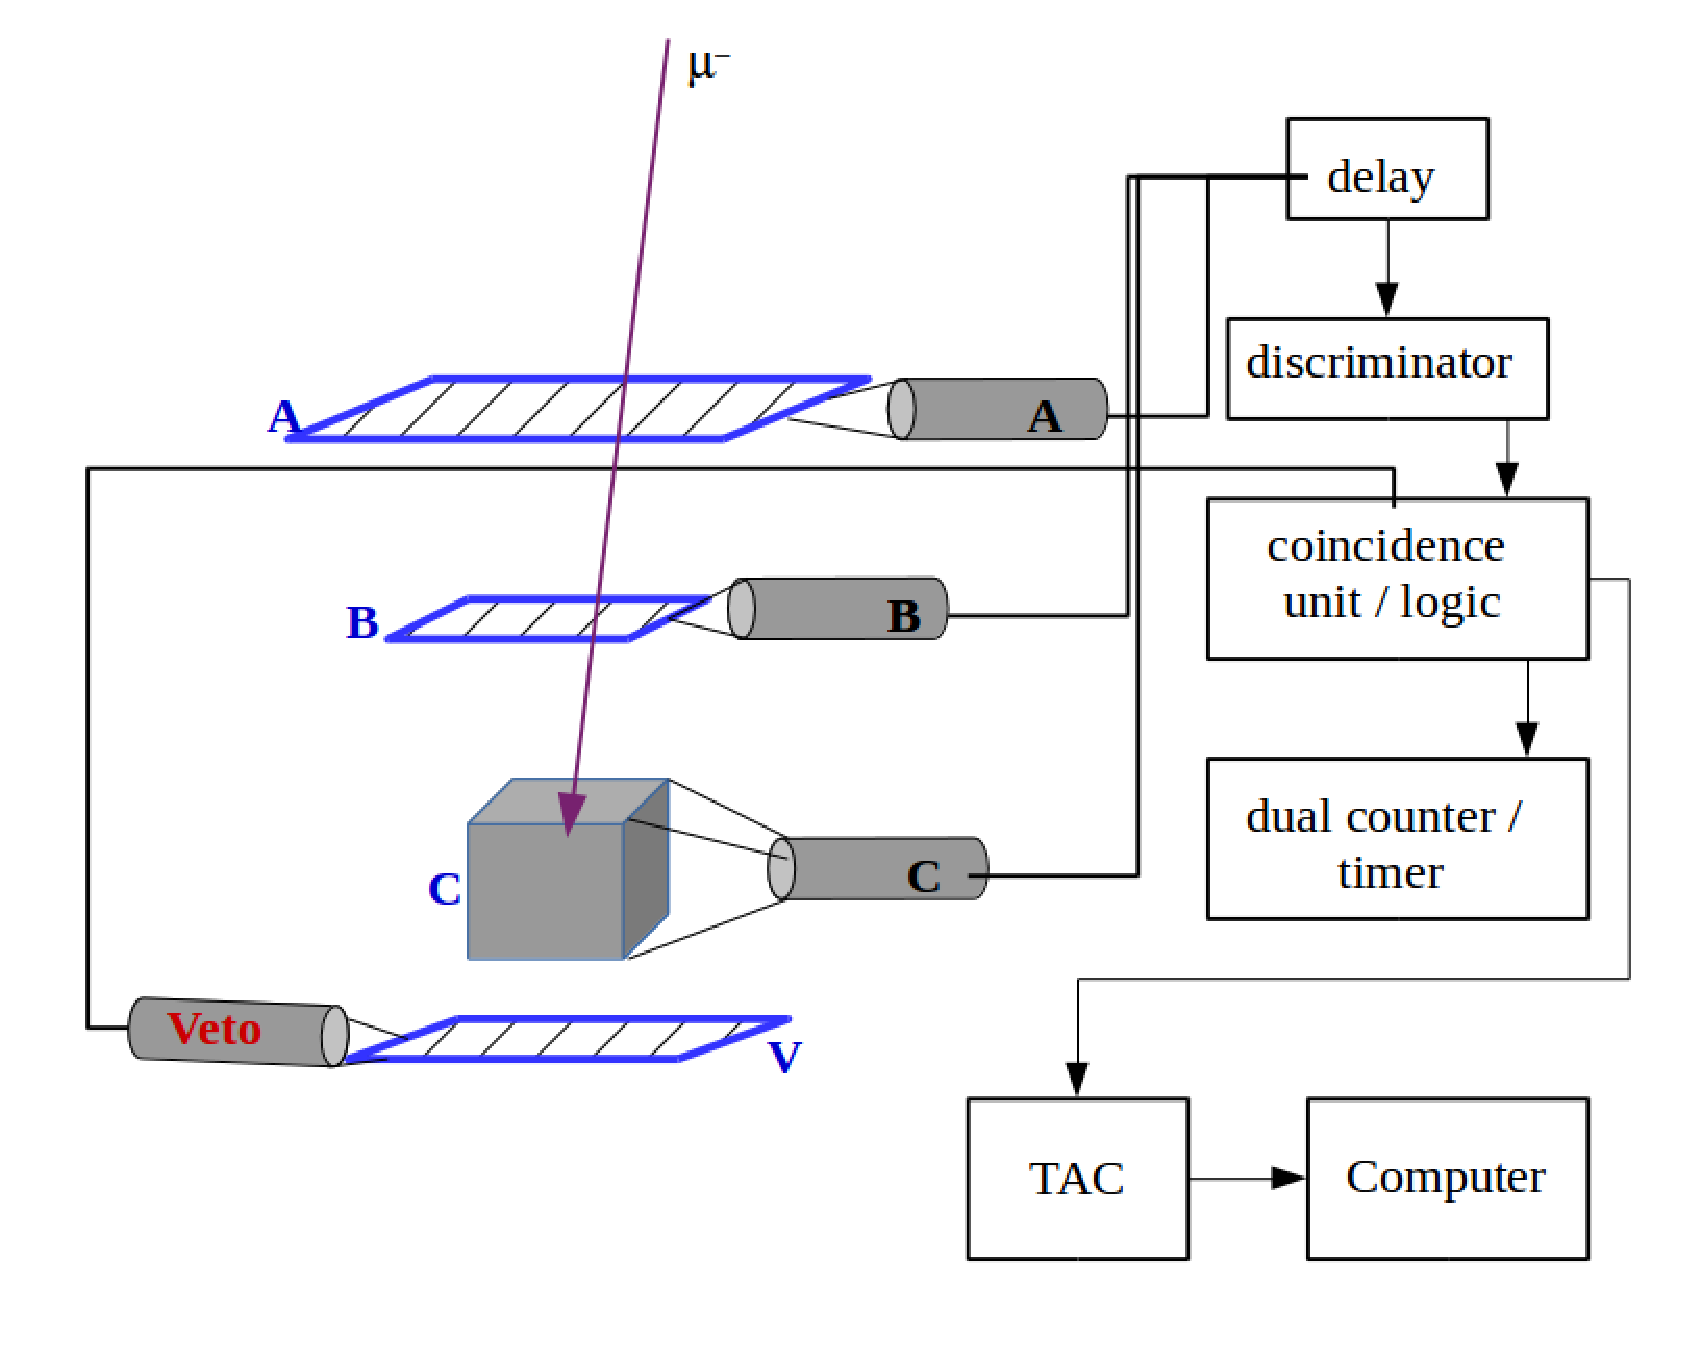
\includegraphics[scale=0.28]{countersetup.eps}
\caption{Schematic diagram of experimental setup: plates A, B, V, and box C are scintillators; PMT tubes are shown as gray cylinders; signals from the PMTs flow through a delay box, then a NIM crate which includes a discriminator, coincidence/logic unit, and dual counter/timer. For $\mu^{-}$ lifetime measurements, logic signals are output to a time to amplitude converter (TAC) and then to a computer for data acquisition. }
\label{Alpha2}
\end{center}
\end{figure}

The muon flux per solid angle is measured with scintillators $A$ and $B$ put into coincidence with delays, and set with a discriminator threshold of approximately 35 mV. Coincidence counts are taken with PMT $A$ and $B$ at a separation of $\Delta r =$ {15.3, 23.0, 37.8, 73.3} cm. In order to obtain the solid angle value with respect to plate $A$, a geometrical correction factor is necessary since plate $B$ is not a point. The plot is given in the appendix. \cite{browder}

Stopped muons in the scintillator box connected to PMT $C$, with plates $A$-$B$ in coincidence and the veto scintillator in anti-coincidence, enables measurements of the particle's lifetime. Delays are adjusted so that the veto signal arrives prior to other signals. Thus in logical expression, measurements start with signals $AB\bar{V}$ and stop with $C$, where $C$ is delayed to avoid through going muons. From the logic output, pulses are sent to a calibrated time amplitude converter (TAC) which measures the time intervals and outputs to a computer for data acquisition via the software called Maestro. \cite{browder} 

To measure the zenith angle dependence of the cosmic ray flux, plates $A$ and $B$ are kept in coincidence and their separation constant. After ensuring all moving parts of the apparatus are fixed, the entire ``telescope'' is rotated thorough the angles $9^{\circ}$, $27^{\circ}$, $45^{\circ}$, $63^{\circ}$, and $81^{\circ}$ with respect to the zenith. \cite{browder}

\begin{figure}[t]
\begin{center}
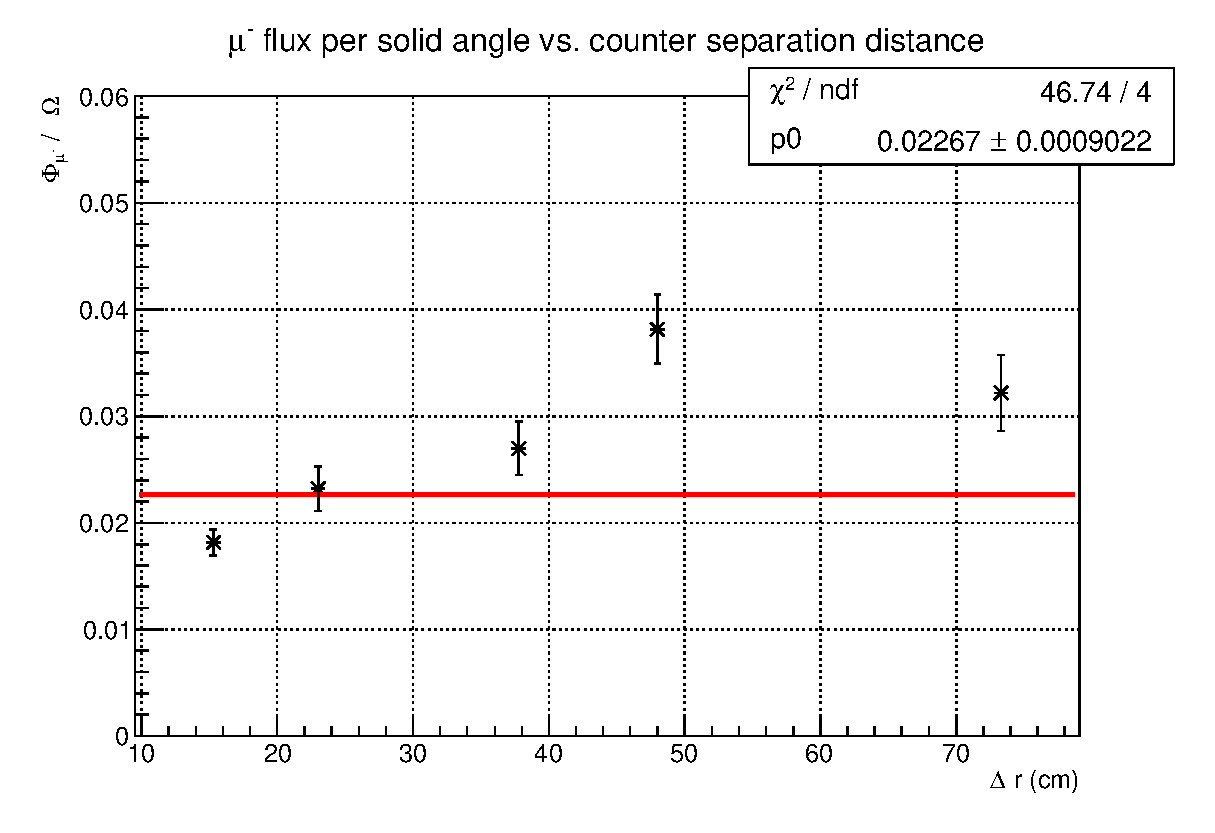
\includegraphics[scale=0.45]{flux_omega.eps}
\caption{The muon flux ($\Phi_{\mu^{-}}$) per solid angle ($\Omega$) as a function of PMT separation ($\Delta r$), where $\Omega$ values are obtained from the plot in figure (5) located in the appendix.}
\label{Alpha2}
\end{center}
\end{figure}

Figure (2) shows muon flux per solid angle at various separations ($\Delta r$) between PMT $A$ and $B$. Due to low statistics, there is large fluctuation about the fitted constant value of $0.023 \pm 0.001$ counts s$^{-1}$cm$^{2}$sr$^{-1}$. Comparing this value to vertical flux of muons given in \cite{pdg}, $\approx .070$ cm$^{-2}$s$^{-1}$sr$^{-1}$, muon flux in the lab is lower due to absorption of atmospheric muons by the surrounding concrete walls.

\begin{figure*}[h]
\begin{center}
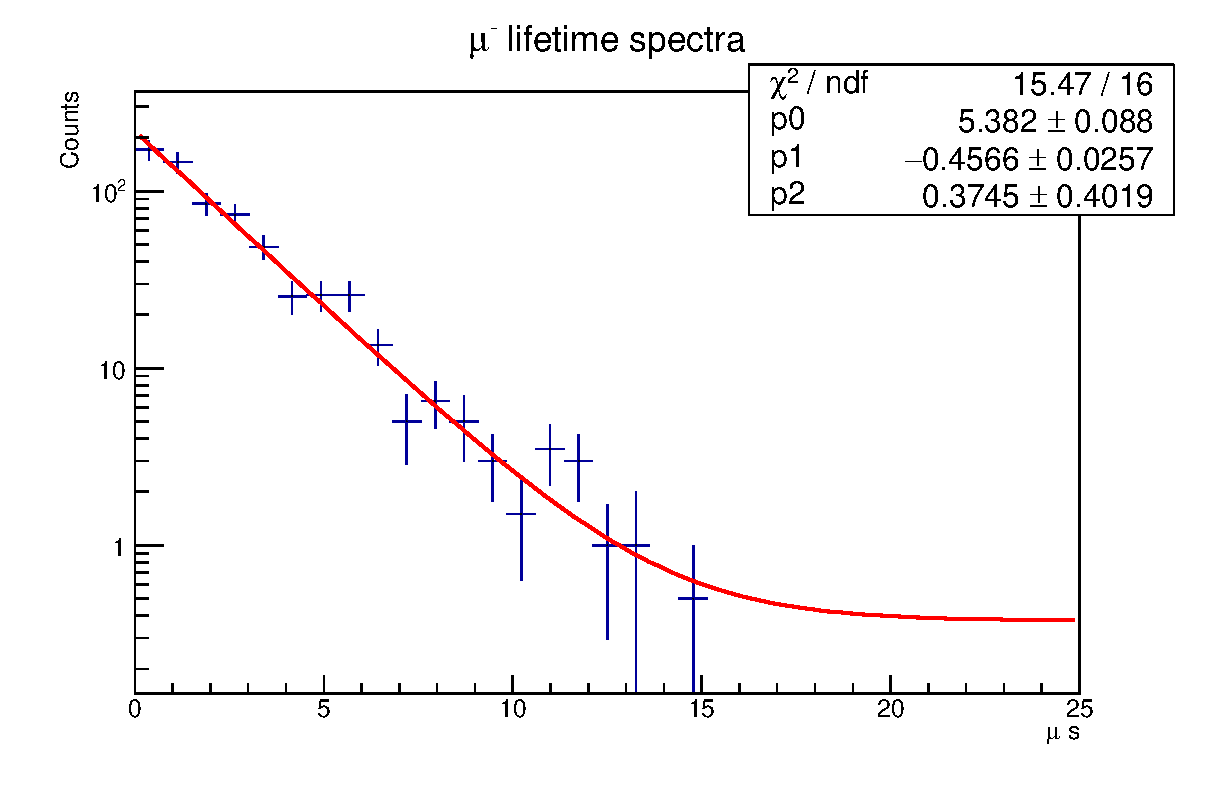
\includegraphics[scale=0.62]{mu_lifetime_final.eps}
\caption{Muon lifetime distribution with and exponential plus constant background fit. Lifetime, given by the inverse of fit parameter p1, is $(2.19 \pm 0.12)$ $\mu$s.}
\end{center}
\end{figure*}
\begin{figure*}[h]
\begin{center}
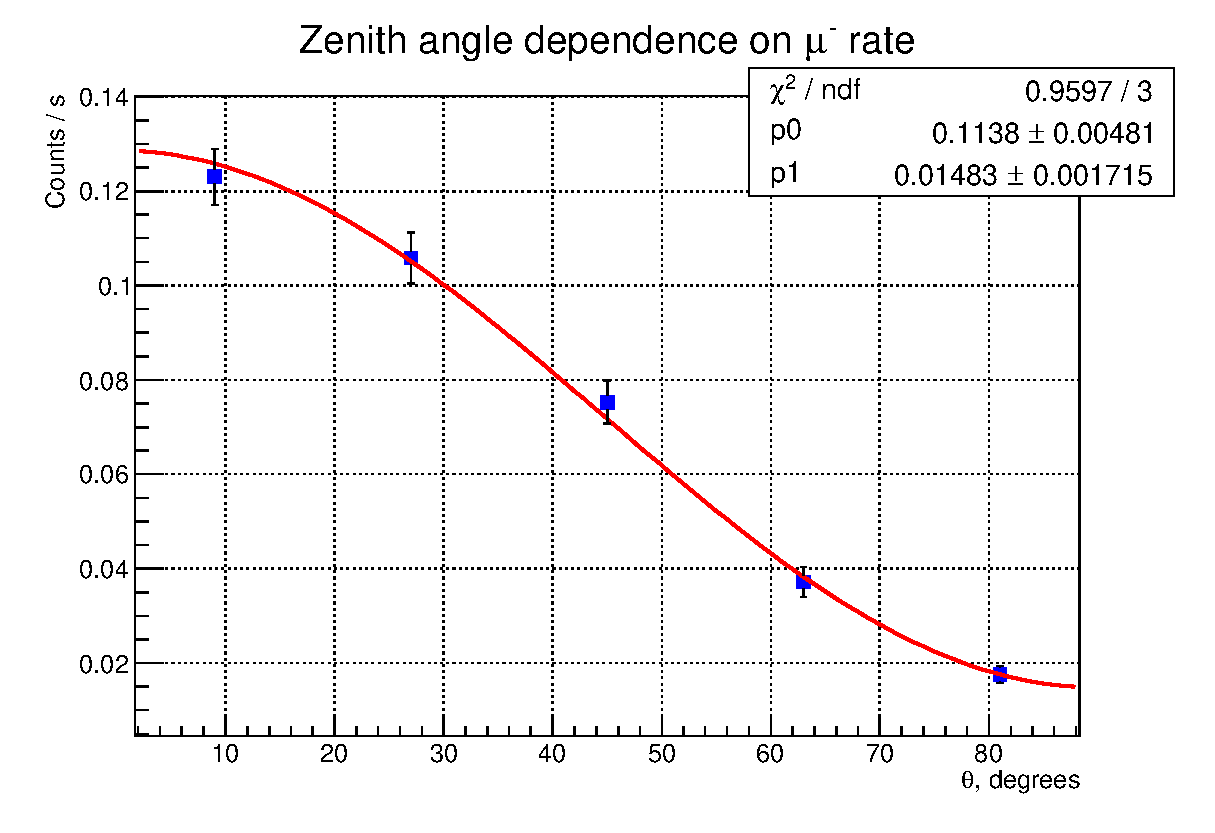
\includegraphics[scale=0.6]{zenith.eps}
\caption{Rotating the ``telescope'' with scintillator plates $A$ and $B$ in coincidence, the muon flux from cosmics is measured at various angles, $\theta$, with respect to the zenith. The angular distribution follows a $cos^2\theta$ distribution.}
\end{center}
\end{figure*}

For the $\mu^{-}$ lifetime measurement data was gathered over the course of 5 days, thus better statistics are obtained. The time distribution of stopped muons is shown in figure (3). The fit to the data is an exponential function with a constant background, where the function is of the form $e^{p0 + p1*x}+p2$. The lifetime is found by taking the inverse of fit parameter p1, and is $(2.19 \pm 0.12)$ $\mu$s. This is in excellent agreement with the known and accepted value of $(2.19703 \pm 0.00004)$ $\mu$s, and well within error. \cite{mass} Errors for counts are taken as Poisson errors and the fit errors are obtained from TMinuit via ROOT. Due to $\mu^{-}$ capture by protons, the measured lifetime is slightly less than free decay. From equation (2) the correction for muon capture in this experiment is found to be approximately $0.32\%$, and is well within the range of experimental uncertainty when compared to the known value of cosmic ray muons on carbon nuclei.\cite{mass}

\begin{equation}
\frac{1}{\tau_e} = \frac{1}{\tau_{\mu}} + \frac{1}{\tau_c}
\end{equation}
The measured decay rate is $1/\tau_e$, and the rates for capture and free decay are respectively $1/\tau_{c}$ and $1/\mu_{\mu}$.


Figure (4) plots the rate of cosmic muons for five different angular positions of the ``telescope'' with respect to the zenith. The fit on the data is the function $p0 cos(x)^2 + p1$, where $p0$ and $p1$ are fit parameters determined via TMinuit in ROOT. The fit is well within statistical and systematic error, and the predicted cosine squared dependence is clear \cite{pdg}.  
  
Given the measured lifetime, it is interesting to calculate the distance it has traveled from say a parent pion with momentum 10 GeV. We take the positively charged pion mass as $m_{\pi} = 139$ MeV/c$^{2}$, the mass of the unstable muon as $m_{\mu} = 105$ MeV/c$^2$, the neutrino as $m_{\nu} = 0$, and use the following equation. 

\begin{equation}
E_{\mu}^2 = m_{\mu}^2 + p_{\mu}^2
\end{equation}

Here $E$, $m$, and $p$ denote the usual energy, mass, and momentum, respectively. Thus, a muon with momentum $\approx 5$ GeV and with lifetime 2.19 $\mu$s, will have a mean decay length of $pt/m \approx 31$ km. This is a stark contrast to the mean decay length of 500 m for a $\pi$ meson with momentum 10 GeV. The physical processes that underly these different behaviors point to the bosons that mediate particle interaction.  

%\begin{nolinenumbers}
\subsection *{Acknowledgement}
\indent \indent
The author wishes to express a special thanks to Dr.Browder and Kevin Croker for providing guidance and excellent physics, and to team members Makana Silva and John Adamski.


\begin{thebibliography}{99}

\bibitem{anderson}
Seth H. Neddermeyer, and Carl D. Anderson. Note on the Nature of Cosmic-Ray Particles. Phys. Rev., Vol. 51, 884. 30 March 1937.

\bibitem{hyper}
http://hyperphysics.phy-astr.gsu.edu/hbase/Particles/muonhist.html

\bibitem{encyc}
http://www.encyclopedia.com/science/enc\\yclopedias-almanacs-transcripts-and-maps/muon-discovery

\bibitem{symm}
http://www.symmetrymagazine.org/\\
sites/default/files/legacy/pdfs/\\201206/muons.pdf
\bibitem{mass}
Adrian C. Melissinos, and Jim Napolitano. Experiments in Modern Physics, 2nd edition. Academic Press 2003. pp. 404-409. 

\bibitem{browder}
http://www.phys.hawaii.edu/~teb/phys481l/\\MuonDecay.txt

\bibitem{pdg}
http://ccwww.kek.jp/pdg/2008/reviews/\\cosmicrayrpp.pdf


\end{thebibliography}

\subsection{Appendix}
\begin{figure}[h]
\begin{center}
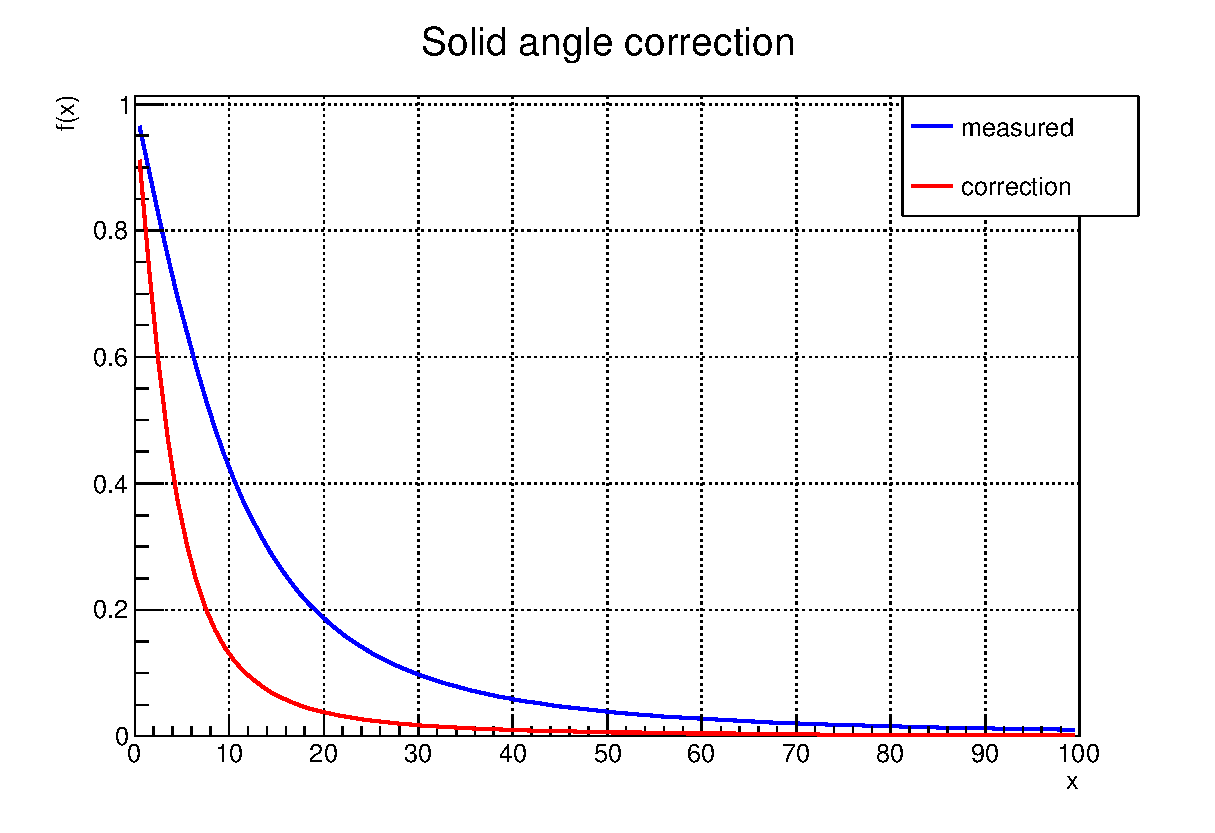
\includegraphics[scale=0.5]{solid.eps}
\caption{Geometrical correction for solid angle calculation where the equation for the solid angle is $f(x) = 4\arccos(-(w^{2}/4)/(h^2+w^2/4))$, and the equation for the solid angle after the correction factor is $f(x) = 4\arccos(-(w^2/4)/(x/b/(w+1))^2 + (w^2/4) - 2\pi))/2\pi$, where $w$ and $b$ are the lengths of the top and bottom square scintillator respectively, $h$ is the height, and $x$ denotes the new effective height. }
\end{center}
\end{figure}


%\end{nolinenumbers}
\end{document}



